\chapter{Related Works} % (fold)
\label{cha:related_works}

% There is a split between different embodiments of robotic systems.
% But, there is also a split between global and local
% planning methods. The global planning methods are usually


\begin{abstract}
In the previous chapter, we have defined \ac{tg} as the problem of finding a
sequence of actions that will move the robot from its current state to a
desired state. As this thesis focuses on \ac{tg} for mobile manipulation,
relevant literature must therefore include works from different fields, ranging
from autonomous driving and mobile robotics to manipulation. Besides, \ac{tg} in
dynamic environments generally includes path planning and local \ac{tg}.
Therefore, this chapter summarizes approaches ordered on a scale of reactivity,
that is the frequency at which trajectories are computed. Starting with
controller-like \ac{tg} methods, we then move in order of increasing
time-horizon up until global path planning.
\end{abstract}


\newpage

% The problem of \ac{tg} is paramount to robotic systems,
% i.e., its solution is required in the context of mobile robots,
% drones, manipulators, and consequently mobile manipulation
% systems. Historicaly, proposed solutions to \ac{tg} were
% developed in parallel for the individual embodiments of
% robotic systems.

\acl{tg} methods aim at finding
global paths that are optimal and collision-free at the
moment of planning. In this section, we review approaches to
\ac{tg} that locally solve the \ac{tg} problem, while aiming
at global optimality --generally not guarnteed-- and
collision avoidance. It is useful to place different methods
on a scale of reactivity, usually measured by the achieved
compute frequency, see \cref{fig:reactivity_scale}.
At the most reactive end, we find low
level controllers and on the least reactive end, we find
global path planning methods.
\begin{figure}[h]
  \centering
  \input{src/state/img/reactivity_scale.pdf_tex}
  \caption{Reactivity scale of different \ac{tg} methods
  revised in this thesis. Global methods, such as RRT
  \cite{Karaman2011} are at the least reactive end. More
  reactive methods, such as \ac{mpc}
  \cite{hewing2020learning}, \ac{apf} \cite{Khatib1985} and
  low-level control methods such as \ac{ic} \cite{hogan1985impedance}
  are at the most reactive end.}
  \label{fig:reactivity_scale}
\end{figure}

\MS{What about learning-based methods?}

\subsection{Impedance control}%
\label{sub:impedance_control}

Impedance control is a widely used control method in
robotics \cite{hogan1985impedance,abu2020variable}. In impedance
control, the controlled system is modeled as a
mass-spring-damper system. The specific case of Cartesian
impedance control was proposed in \cite{albu2002cartesian} and
could be characterized as a local \ac{tg} method, because of
its ability cope with various goal specifications and its
safety properities in the proximity of humans
~\cite{van2022disagreement,hjorth2024enabling}.
Additionally, impedance control can be used in collaborative
settings, e.g., when lifting large objects together with
humans \cite{abu2020variable}. More recent works on
impedance control use variable impedance parameters to adapt
the robot's behavior to the task at hand
\cite{abu2020variable}. Often, the impedance controller are
modified by human feedback to improve perceived safety and
increase reliablity of the task exeuction with human
feedback \cite{lachner2022shaping,franzese2021ilosa}.

\subsection{Reactive trajectory generation}%
\label{sub:reactive_trajectory_generation}

In this dissertation, we refer to \textit{reactive \ac{tg}}
as methods that rely on local information about the
environment and the robot that compute actions without a
time horizon into the future. The most prominent example of
reactive \ac{tg} is the \ac{apf} method as we will
see by visiting the different embodiments of robotic
systems.

\subsubsection{Robotic arms}
\label{subsub:robotic_arms}

Pioneer works on \ac{tg} for robotic arms
employed \ac{apf} for collision avoidance
\cite{Khatib1985,Khatib1986real,park2008movement}. Building
on the previous, \cite{Haddadin2011} introduced the Circular
Field method to address dynamic collision avoidance. To
ensure collision avoidance for the end-effector when
grasping a moving obstacle, \cite{Du2018} employed a
repulsive vector.
Velocity scaling of trajectories in the presence of 
contact forces was addressed in \cite{haddadin2010real}.

Reactive \ac{tg} can also be formulated as an optimization
problem. In this case, the optimization problem is solved
at each time step. While statements about global optimality
are not possible, different objectives can be encoded in the
cost function and avoidances can be integrated using
constraints. By maximizing manipulability the robot remains
flexible to changes in the environment while reaching a goal
pose \cite{haviland2020purely}. The work was later extended
to integrate moving and static obstacles
\cite{haviland2021neo}.

\subsubsection{Mobile robots}
\label{subsub:mobile_robots}

The method of \ac{apf} was also used for \ac{tg} of mobile
robotis after its introduction for robotic arms.
For non-holonomic mobile robots, it was shown that \ac{apf}
generally exhibits multiple equilibrium points which are not
necessarily stable \cite{urakubo2018stability}.

Different to \ac{apf}, the dynamic window approach searches
the space of feasible velocities and computes the best
velocity command for the next time step
\cite{fox1997dynamic}. This methods was extended to take
into consideration global reference paths
\cite{zhang2019improved}.

\subsubsection{Mobile Manipulators}
\label{subsub:mobile_manipulators}

\MS{Does not seem to exist...}



\subsection{Receding-horizon trajectory optimization}%
\label{sub:receding_horizon_trajectory_optimization}

Methods formulating local \ac{tg} as an optimization problem with a finite
discrete time horizon are known under the name of receding-horizon trajectory
optimization. In line with most literature in robotics, we will refer to such
methods as \ac{mpc}.
Generally, several objectives are encoded in the scalar cost function, dynamics
are formulated as equality constraints and inequality constraints ensure
collision avoidance and joint limit avoidance. The dynamics for this problem can
include the full dynamics model or simple integrating
schemes \cite{hewing2020learning}.
By explicitly solving the constrained optimization problem, this approach yields
formal guarantees on stability. Stability for \ac{mpc} is proven by formulating
an appropriate Lyapunov function and showing that the finite time-horizon
formulation with an appropriate terminal cost results in the same stability as
the corresponding infinite time-horizon formulation
\cite{l1,l4,keerthi1988optimal}. 

Despite these results, formal stability
guarantees in such environments are challenging as appropriate terminal cost
functions are often not computable or too conservative. Besides, the
computational costs scale with the degrees of freedom restricting real-time
applicability to simple dynamics and environment models \cite{Spahn2021}.

Some \ac{mpc} formulations are non-linear and can be analyzed
using methods from non-linear control. When analyzing non-linear control
system, Riemannian energies lead to more detailed stability results than
Lyapunov functions. By investigating the variation around the generated
trajectory and its contracting towards the desired trajectory, some control
designs show exponential stabilizing properties \cite{l2}. These
findings have been applied to tracking control problems \cite{l3}.

\subsubsection{Mobile robots}
\label{subsub:mobile_robots}

The dynamic window approach \cite{Fox1997} and its new variant proposed in
\cite{Zhang2019} have proven to be efficient in generating smooth trajectories
for mobile robots in static and dynamic environments. To navigate among
pedestrians, \cite{Ferrer2013} introduced the Social Forces model imitating
the human navigation behavior and using it as navigation policy for the
robot.  Yet, Social Forces and its variants rely on handcrafted functions
limiting their ability to handle more complex navigation scenarios. To deal
with a large number of agents, \textit{ORCA} was proposed in
\cite{VanDenBerg2011} and later extended for non-holonomic bases in
\cite{Alonso-Mora2012a}. However, these approaches demonstrate highly reactive
behaviors because they only consider one step look-ahead predictions.

MPC schemes were proposed for mobile robots and autonomous vehicles in
\cite{Brito2019} and \cite{Schwarting2018} allowing to optimize over a
prediction horizon and avoid, in advance, dynamic obstacles.  Several 3D MPC
formulation were proposed for drones to enable safe motion through cluttered
environments \cite{Tordesillas2019,Liu2017}.

\subsubsection{Robotic arms}
\label{subsub:robotic_arms}

Early implementations of \ac{mpc} for industrial robotics
arms were presented in \cite{faulwasser2016implementation}.
Especially in the context of robotic arms, uncertainty in
the robot model might harm the performance. To overcome this
limitation, Gaussian Processes were proposed in
\cite{hewing2019cautious,carron2019data} to offline learn
the mismatch between model and real system. The learned
model was then used to adapt the \ac{mpc} scheme during
runtime \cite{carron2019data}.

\subsubsection{Mobile Manipulators}
\label{subsub:mobile_manipulators}

In the context of mobile manipulation, less research focused on collision
avoidance in dynamic environments, including changing scenes and moving
obstacles. A real-time controller using MPC was presented in \cite{Ide2011}, in
which either a holonomic or a non-holonomic base was combined with a
two-degree-of-freedom robotic arm mounted onto the base. Although hardware
constraints were respected, no collision avoidance was considered.  An MPC
formulation for mobile manipulators with holonomic bases that allows collision
avoidance was presented in \cite{Avanzini2015}. The perceived obstacles were
translated into a set of spheres to be respected by the MPC scheme. The proposed
approach used dynamically changing weights to change between arm motion and
locomotion, resulting in a locked arm during navigation. A different weight
setting was used to perform motion underneath a horizontal bar with an a priori
position. The work is extended to non-holonomic bases and includes object
detection in moving underneath the horizontal bar \cite{Avanzini2018}. 


\subsubsection{Conclusion}

Receding-horizon trajectory optimization methods are a
powerful tool for local \ac{tg} in dynamic environments.
They provide formal stability guarantees and can be analyzed
using methods from non-linear control. Therefore, \ac{mpc}
approaches are widely used in the context of autonomous
driving. For manipulators, model inaccuracies degrade
performance and learning methods are often used to
compensate for this. However, the computational costs scale
with the degrees of freedom and restrict real-time
applicability to simple dynamics and environment models.

\section{Path planning}
\label{sec:path_planning}

Past works devoted to path planning can be divided into two
main categories: optimization-based and sampling-based
methods \cite{LaValle2006,Mukadam2017}. Sampling-based path
planners generate random configurations until a valid path
between an initial configuration and a set of goal
configurations is found \cite{Karaman2011}. Sampling-based
methods, such as rapidly exploring random trees (RRT's)
\cite{Webb2013,Kleinbort2019,Kuffner2000} and probabilistic
roadmaps (PRM's) \cite{Hsu2002,Faust2017} are highly
efficient at generating paths for systems with high-degree
of freedom.

\subsection{Robotic arms}%
\label{sub:robotic_arms}

Motion planning problems are usually defined by goals in
arbitrary task spaces, such as the 3D Euclidean space or
end-effector poses. For mobile robots, where task space and
configuration space are often identical \cite{LaValle2006},
the mapping from task space to configuration space is
straightforward. However, in the context of manipulation,
tasks can be regarded as constraints to the motion planning
problem. Conventional approaches to motion planning rely on
inverse kinematics to transform task constraints into sets
of configurations. The resulting path planning problem can
then be solved using sampling-based methods
\cite{Rickert2014}.

Several methods have been proposed to
directly integrate task constraints into the sampling phase.
\cite{Stilman2010} proposed a method to iteratively push a
random sample to the manifold adhering to the task
constraint. The notion of task constraints was later
extended to task space regions to define soft constraints
for individual task components~\cite{Berenson2011}.
\cite{Kingston2019} proposed scalar-valued functions to
represent task constraints for sampling-based planning. As
all of the above-mentioned methods rely on implicitly
constrained sampling in the joint space, they exhibit high
computational time, which is especially harmful to
real-world applications \cite{qureshi2021constrained}.

\subsection{Mobile Manipulators}
\label{sub:mobile_manipulators}

Despite abundant research in trajectory planning for mobile robots and robotic
arms, few works focused on coupling both systems' control. It was shown that
coupling the base and the robotic arm motion leads to a considerable reduction
of total operational time and smoother motions \cite{Thakar2018, Thakar2019}.
Nevertheless, these methods were designed for static environments and did not
allow real-time collision avoidance. Furthermore, trajectory planning for the
coupled system is a precondition for effective interactive navigation, including
opening doors \cite{Jain2009, Chitta2010} or moving obstacles out of the way
\cite{Li2019}.

To summarize, path planning in robotics is a well-studied
problem. Especially in the early days of robotics, where
robots were mostly deployed in static environments, path
planning was a central problem. However, when exposed to
dynamic environments, path planning becomes insufficient due
to its unability to quickly react to changes in the
environment. This is especially true for mobile manipulation
systems, due to their high-dimensional configuration space,
\cite{Avanzini2018}. To overcome this limitation, local
trajectory generation methods have been proposed as we will
see in the next section.



\subsection{Geometries of trajectories}
\label{sub:geometries_of_trajectories}

Reactive \ac{tg} approaches, such as \ac{apf} theory,
may lead to contracting behaviors, as individual policies
are \textit{fighting} against each other \cite{Ratliff2018}.
To overcome the shortcoming, importance metric and policy
are decoupled in \ac{rmp}. This tuple defines
for each \textit{behavior} a dynamical system.
Defining collision avoidance behavior as dynamical systems
is a widely used approach
\cite{khansari2012dynamical,huber2023avoidance}, for which
\ac{osc} \cite{Khatib1987a} and \ac{dmp}
\cite{ijspeert2013dynamical} are special cases.


\MS{That is still out of place.}
Based on the findings of contracting metrics for non-linear
control design \cite{l2,l3}, geometric control approaches design the motion
generation such that convergence is inherent to the problem formulation
rather than imposing them on the solution process. Practically, individual
constraints to the motion planning problem shape the optimization manifold
so that the solution is accessible through the solution of simple differential
equation. An example for shaping the optimization
manifold is seen in \cref{fig:spec_combination}.

%
\begin{figure}[h]
  \centering
  \begin{subfigure}{0.33\linewidth}
    \centering
    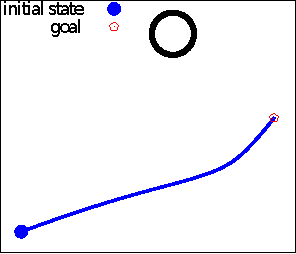
\includegraphics[width=0.9\textwidth]{state/trajectory_obst2}
    \caption{}
    \label{subfig:trajectory_obst1}
  \end{subfigure}%
  \begin{subfigure}{0.33\linewidth}
    \centering
    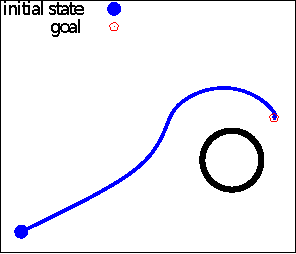
\includegraphics[width=0.9\textwidth]{state/trajectory_obst1}
    \caption{}
    \label{subfig:trajectory_obst2}
  \end{subfigure}%
  \begin{subfigure}{0.33\linewidth}
    \centering
    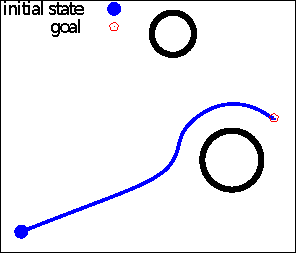
\includegraphics[width=0.9\textwidth]{state/trajectory_both_obstacles}
    \caption{}
    \label{subfig:trajectory_both_obstacles}
  \end{subfigure}
  \caption{
    Combining different avoidance behaviors using optimization fabrics. The
    components defining collision avoidance with single obstacles (a,b) are
    combined in (c). Obstacles are shown in black. Trajectories of the point
    robot are shown in blue.
  }
  \label{fig:spec_combination}
\end{figure}
%
Realizing this concept, Riemannian motion policies (RMPs) represent a
natural way of combining multiple policies into one joined policy.
RMPs define individual sub-tasks of the motion planning as
differential equations (\textit{spectral semi sprays} or
\textit{specs} for short) of second order and propose the
\textit{pullback} and \textit{summation} operators to combine multiple policies
in the configuration space. As subtasks can be defined in arbitrary manifolds
of the configuration space, RMP generalize operational space
control~\cite{Khatib1987}. The resulting behavior of RMP was reported to be
intuitive while keeping computational costs low~\cite{Ratliff2018}. The concept
of RMP was used in~\cite{Cheng2018,Cheng2020} to form RMP-Flow, a motion
planning algorithm that is shown to be conditionally stable and invariant
across robots. In RMP-Flow, individual tasks are represented as a pair of
a motion policy and a corresponding metric defining the importance of
individual directions. An RMP adaptation was proposed for non-holonomic robots
in~\cite{Meng2019}. By incorporating the kinematic constraint into the root
equation of the RMP, the computed policy is applicable to non-holonomic robots.
Besides, that work proposed a neural net to learn the collision avoidance task
components. 

Although RMPs have proven to be a powerful tool for
motion generation, it was reported to require intuition and experience
during tuning~\cite{Ratliff2020}. Optimization fabrics with Finsler structures
as metric generators simplify the motion design as the conditions for stability
and convergence are inherent to the definition of Finsler
structures~\cite{Ratliff2020,Ratliff2021}. Opposed to RMPs, where the metric is
typically user-defined, fabrics derive Finsler metrics from artificial
energies, similar to approaches from control design, \cite{l2,l3}, using the
Euler-Lagrange-Equation from geometric mechanics. Although fabrics generalize
the concept of RMPs and make it accessible to a broader audience by
decreasing the intuition and expertise required, they have not yet been applied
to a wide range of robots. 

The reason for this lack of application of fabrics is twofold. First, all the
above mentioned methods are reactive and highly local methods, thus making them
prone to local minima \cite{Bhardwaj2021}. As RMPs and optimization
fabrics do not incorporate path following, integration of global
planning to overcome local minima is not possible to this date. Second, fabrics
and RMP do not make use of velocity estimates of obstacles but rely purely on
their high reactivity in dynamic environments. As for other trajectory
optimization techniques, motion estimates could benefit fabrics (and RMP) to
result in even smoother motion and allow applications in such environments. 

\subsection{Mobile robots}
\label{sub:mobile_robots}


\subsection{Robotic arms}
\label{sub:robotic_arms}



\subsubsection{Mobile Manipulators}
\label{subsub:mobile_manipulators}

